\section{Erkennungsgenauigkeit}
Es werden 3 Features näher betrachtet. Motion History, Helligkeitsverteilung und Schwerpunktverteilung. Aus denen werden 6 Featuremengen generiert, die zum Trainieren genutzt werden. Insgesamt wurden X(TODO)
verschiedene Konfigurationen trainiert und getestet (siehe Sektion \ref{sec:Training}).
\newline
\newline
Betrachtet wird die beste Konfiguration, die innerhalb der Restriktion des Programmspeichers, nach möglichen Optimierungen (siehe Sektion \ref{sec:eval_size}), die Summe der Erkennungsgenauigkeiten
der Testmenge von Klisch und der Nullgestentestmenge maximiert.
\newline
\newline
Die verschiedenen Featuremengen werden im Hinblick auf die Erkennungsgenauigkeit auf der Testmenge von Klisch, der Nullgestentestmenge, der neuerstellten Gestentestmenge und der synthetischen
Helligkeitstestmenge untereinander verglichen. Außerdem wird die Auswirkung von verschiedenen Baumhöhen und Waldgrößen untersucht. Zuletzt wird die beste Konfiguration mit den Ergebnissen von Giese verglichen.

\subsection{Helligkeitsverteilung}
\begin{table}[h!]
    \centering
    \begin{tabular}{ | l | c | c | c |}
        \hline
        Konfiguration & Beste & Unter 44 kB & Unter 28 kB \\\hline
        Ensemble-Methode & ExtraTrees & ExtraTrees & ExtraTrees \\\hline
        Maximalhöhe & 14 & 10 & 15 \\\hline
        Waldgröße & 10 & 6 & 1 \\\hline
        Blattgröße (min\_samples\_leaf) & 4 & 4 & 4 \\\hline
        Programmgröße in Bytes & 76628 & 33284 & 9364 \\\hline
        Genauigkeit Testmenge von Klisch & 74,0\% & 63,5\% & 67,7\% \\\hline
        Genauigkeit Gestentestmenge & 74,1\% & 79,2\% & 76,6\% \\\hline
        Genauigkeit Nullgestentestmenge & 69,0\% & 71,0\% & 67,0\% \\\hline
    \end{tabular}
    \caption{Die beste Konfigurationen der Helligkeitsverteilung.}
    \label{tab:helligkeitsverteilung}
\end{table}
\begin{figure}[h!]
    \centering
    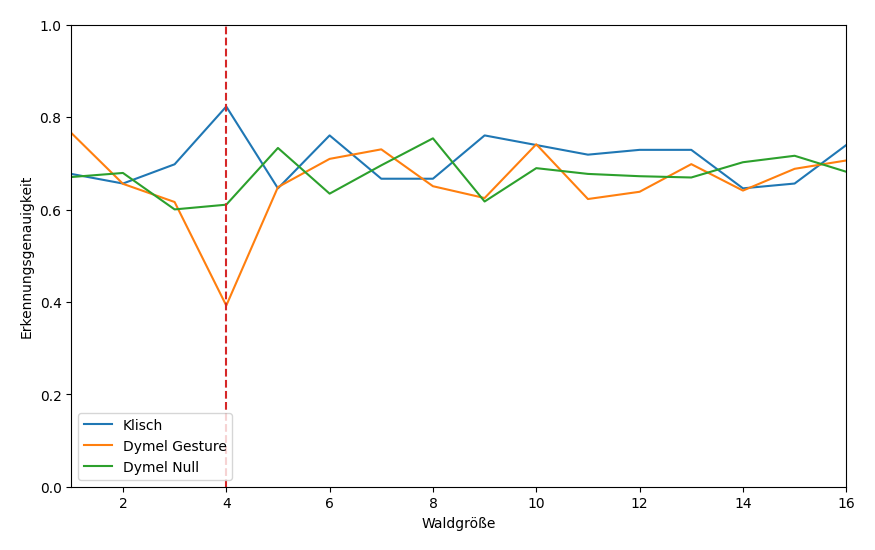
\includegraphics[width=\linewidth]{images/helligkeitsverteilung_acc_per_size.png}
    \caption{Die besten Konfigurationen pro Waldgröße mit der Helligkeitsverteilung.}
    \label{fig:helligkeitsverteilung_per_forest_size}
\end{figure}
Die Featuremenge der Helligkeitsverteilung beinhaltet insgesamt 12 Features. Jeweils 6 Feature repräsentieren Zeitfenster der minimalen Helligkeit und der maximalen Helligkeit. Die Zeitfenster wurden
geometrisch zusammengefasst.
\newline
\newline
Aus der Tabelle \ref{tab:helligkeitsverteilung} sind die besten Konfigurationen jeder Kategorie zu entnehmen. Die beste Konfiguration wurde mit der Ensemble-Methode \textit{ExtraTrees} gefunden.
Sie erzielt eine Klassifizierungsgenauigkeit von 74\% auf der Testmenge von Klisch und ist damit 25,2\% schlechter als das neuronale Netzwerk von Giese \cite{gieseThesis}. Außerdem wird 74\% der Gestentestmenge
und 69\% der Nullgestentestmenge korrekt klassifiziert.
\newline
\newline
Wird die Kategorie \textit{Beste} und die Kategorie \textit{Unter 28 kB} vergleichen, nimmt die Gesamtklassifizierungsgenauigkeit nur um 1,94\% ab. Dabei reduziert sich die Programmgröße um 87,8\%.
Ein ähnliches Verhalten ist auch in Abbildung \ref{fig:helligkeitsverteilung_per_forest_size} zu erkennen. Dort ist nur ein geringer Zuwachs der Gesamtklassifizierungsgenauigkeit mit der zunehmenden
Waldgröße zu beobachten.
\subsection{Motion History}
\begin{table}[h!]
    \centering
    \begin{tabular}{ | l | c | c | c |}
        \hline
        Konfiguration & Beste & Unter 44 kB & Unter 28 kB \\\hline
        Ensemble-Methode & ExtraTrees & ExtraTrees & ExtraTrees \\\hline
        Maximalhöhe & 10 & 11 & 9 \\\hline
        Waldgröße & 16 & 7 & 6 \\\hline
        Blattgröße (min\_samples\_leaf) & 1 & 2 & 1 \\\hline
        Programmgröße in Bytes & 84200 & 40456 & 22804 \\\hline
        Genauigkeit Testmenge von Klisch & 68,8\% & 67,7\% & 62,5\% \\\hline
        Genauigkeit Gestentestmenge & 74,5\% & 67,6\% & 68,5\% \\\hline
        Genauigkeit Nullgestentestmenge & 68,3\% & 64,4\% & 67,6\% \\\hline
    \end{tabular}
    \caption{Die besten Konfigurationen der Feature-Menge Motion History.}
    \label{tab:motion_history}
\end{table}
\begin{figure}[h!]
    \centering
    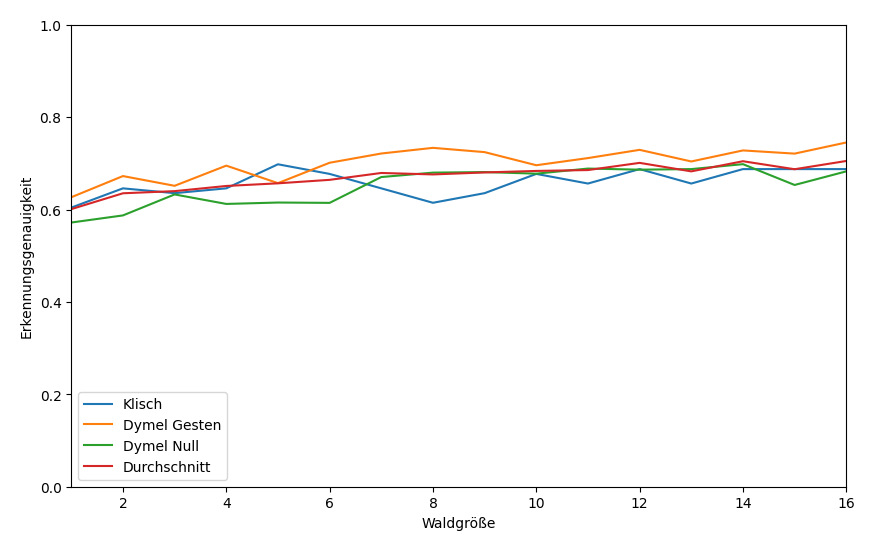
\includegraphics[width=\linewidth]{images/motion_history_acc_per_size.png}
    \caption{Die besten Modelle pro Waldgröße der Feature-Menge Motion History.}
    \label{fig:motion_history_per_forest_size}
\end{figure}
Die Feature-Menge Motion History beinhaltet für jeden Pixel ein Feature, das der Definition des Motion History Image folgt (Formel \ref{formular:mhi}), wobei $\tau=100$ und $\delta=\frac{\tau}{\#Bilder}$ ist.
\newline
\newline
Aus Tabelle \ref{tab:helligkeitsverteilung} sind die besten Konfigurationen jeder Kategorie zu entnehmen. Die beste Konfiguration wurde wieder mit der Ensemble-Methode \textit{ExtraTrees} gefunden.
Das Modell erzielt eine Klassifizierungsgenauigkeit von 68,8\% auf der Testmenge von Klisch, 74\% auf der Gestentestmenge und 69\% auf der Nullgestentestmenge. Im Vergleich zu der Helligkeitsverteilung
wird mehr Programmspeicher benötigt und die Gesamtklassifizierungsgenauigkeit ist 1,84\% schlechter.
\newline
\newline
Wird die Kategorie \textit{Beste} mit der Kategorie \textit{Unter 28~kB} verglichen, nimmt die Gesamtklassifizierungsgenauigkeit nur um 4,3\% ab. Dabei reduziert sich die Programmgröße um 72,9\%.
Abbildung \ref{fig:motion_history_per_forest_size} zeigt, dass die Klassifizierungsgenauigkeit im Durchschnitt sich mit zunehmender Waldgröße erhöht. Im Vergleich zur Helligkeitsverteilung, ist der Zuwachs größer.
Wenn der Suchraum nicht auf eine Waldgröße von 16~Bäumen begrenzt wäre, würde die beste Konfiguration vermutlich besser sein. Allerdings würde sich auch die Programmgröße signifikant erhöhen.
\newline
\newline
Die Motion History kann mit ausschließlich 8-Bit Integer implementiert werden und hat damit die geringste WCET und Programmgröße pro Baum, weswegen die beste Konfiguration mit einer Waldgröße von 16~Bäumen nicht deutlich
größer ist, als die der Helligkeitsverteilung mit einer Waldgröße von 10~Bäumen.

\subsection{Brightness Distribution and Motion History}
Show graphs about:
Best solution,
Best feasible solution,
With and WithOUT considering null gestures.
Talk when it starts to generalize more poorly(?)

\subsection{Schwerpunktverteilung mit Gleitkommazahlen}
\begin{table}[h!]
    \hspace{-0.5cm}
    \begin{tabular}{ | l | c | c | c | c |}
        \hline
        Konfiguration & Beste & Unter 60 kB & Unter 28 kB & Unter 14 kB \\\hline
        Ensemble-Methode & Boosting & Boosting & RandomForest & Bagging  \\\hline
        Maximalhöhe & 20 & 19 & 10 & 7 \\\hline
        Waldgröße & 10 & 6 & 4 & 3 \\\hline
        min\_samples\_leaf & 8 & 8 & 2 & 8 \\\hline
        Programmgröße in Bytes & 83304 & 43678 & 20188 & 6656 \\\hline
        Genauigkeit Testmenge von Klisch & 94,8\% & 94.8\% & 89,6\% & 87,5\% \\\hline
        Genauigkeit Gestentestmenge & 97,0\% & 96,1\% & 95,6\% & 94,1\% \\\hline
        Genauigkeit Nullgestentestmenge & 92,2\% & 91,1\% & 88,8\% & 89,9\% \\\hline
    \end{tabular}
    \caption{Beste Konfigurationen der Schwerpunktverteilung mit Gleitkommazahlen.}
    \label{tab:schwerpunktverteilung_float}
\end{table}
\begin{figure}[h!]
    \centering
    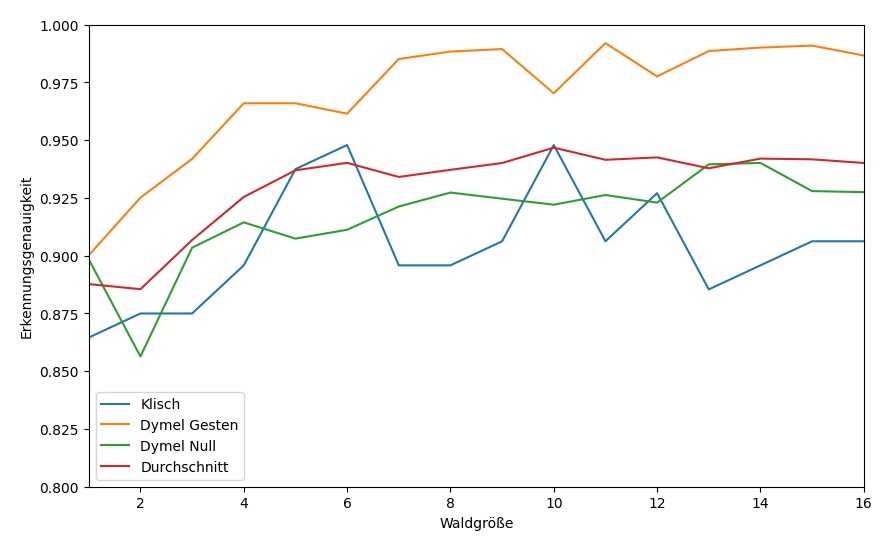
\includegraphics[width=\linewidth]{images/cocd_float_acc_per_size.png}
    \caption{Die beste summierte Erkennungsgenauigkeit pro Waldgröße der Schwerpunktverteilung mit Gleitkommazahlen.}
    \label{fig:cocd_float_per_forest_size}
\end{figure}
Die Featuremenge Schwerpunktverteilung mit Gleitkommazahlen folgt der Definition aus Sektion \ref{sec:schwerpunktverteilung} und beinhaltet insgesamt 10 Einträge, wobei jeweils 2 Einträge die X und Y
Koordinate des Schwerpunktes darstellen in insgesamt 5 Zeitfenstern.
\newline
\newline
Die beste Konfiguration wurde mit der Ensemble-Methode Boosting erzielt (siehe Tabelle \ref{tab:schwerpunktverteilung_float}). Mit einer Erkennungsgenauigkeit von 94,8\% auf der Testmenge von Klisch
ist dieser Ansatz nur 5,2\% schlechter als das neuronale Netz von Giese \cite{gieseThesis}. Es ist anzumerken, dass mit einer kleineren Trainingsmenge ohne die Gestentrainingsmenge und Nullgestentrainingsmenge eine Lösung
gefunden wurde, die 97,9\% erzielte und damit nur 2,1\% schlechter ist. Außerdem werden 97\% der Gestentestmenge und 92,2\% der Nullgestentestmenge korrekt klassifiziert.
\newline
\newline
Im Vergleich zu der Helligkeitsverteilung und Motion History ist die Erkennungsgenauigkeit dieses Ansatzes signifikant besser, sogar wenn nur 6656 Byte Programmspeicher verwendet werden. Wird die beste Konfiguration mit
der \textit{Unter 14 kB} verglichen, nimmt die Gesamterkennungsganuigkeit nur um 4,17\% ab bei der Reduktion der Programmgröße von 92\%. Dies verspricht, dass mit zunehmender Waldgröße der die Erkennungsgenauigkeit steigt.
Abbildung \ref{fig:cocd_float_per_forest_size} zeigt, dass dies zwar der Fall ist, aber schon ab einer Waldgröße von 6 ist die Durchschnittliche Erkennungsgenauigkeit keinen signifikanten Zuwachs mehr verzeichnet.
Dementsprechend ist der Unterschied der Gesamterkennungsgenauigkeit der besten Konfiguraiton und \textit{Unter 60 kB} mit 0,7\% nicht groß, wodurch sich dieses Feature gut für kleine eingebettete Systeme mit
wenig Programmspeicher eignet.
\subsection{Schwerpunktverteilung mit Ganzzahlen}
\begin{table}[h!]
    \hspace{-0.5cm}
    \begin{tabular}{ | l | c | c | c |}
        \hline
        Konfiguration & Beste & Unter 44 kB \& 28 kB & Unter 14 kB \\\hline
        Ensemble-Methode & ExtraTrees & Random Forest & Random Forest \\\hline
        Maximalhöhe & 21 & 13 & 12 \\\hline
        Waldgröße & 11 & 7 & 3 \\\hline
        Blattgröße (min\_samples\_leaf) & 2 & 4 & 1 \\\hline
        Programmgröße in Bytes & 76200 & 21532 & 11012 \\\hline
        Genauigkeit Testmenge von Klisch & 95,8\% & 91,7\% & 86,5\% \\\hline
        Genauigkeit Gestentestmenge & 98,8\% & 97,1\% & 95,5\% \\\hline
        Genauigkeit Nullgestentestmenge & 95,6\% & 94,5\% & 88,9\% \\\hline
    \end{tabular}
    \caption{Die besten Konfigurationen der Schwerpunktverteilung mit Ganzzahlen.}
    \label{tab:schwerpunktverteilung_int}
\end{table}
\begin{figure}[h!]
    \centering
    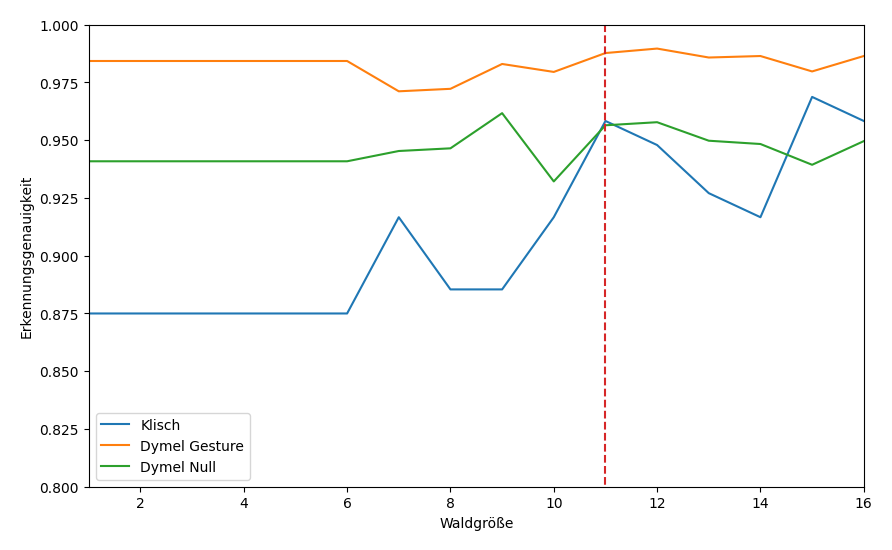
\includegraphics[width=\linewidth]{images/cocd_int_acc_per_size.png}
    \caption{Die besten Konfigurationen pro Waldgröße der Schwerpunktverteilung mit Ganzzahlen.}
    \label{fig:cocd_int_per_forest_size}
\end{figure}
Die Featuremenge Schwerpunktverteilung mit Ganzzahlen folgt der Definition aus Kapitel \ref{sec:schwerpunktverteilung} und beinhaltet insgesamt 10 Einträge. Jeweils 2 Einträge bilden die X und Y
Koordinate des Schwerpunktes. Damit spiegeln 10 Einträge insgesamt 5 Zeitfenster wieder.
\newline
\newline
Aus der Tabelle \ref{tab:schwerpunktverteilung_int} sind die besten Konfigurationen jeder Kategorie zu entnehmen. Die beste Konfiguration wurde mit der Ensemble-Methode ExtraTrees gefunden.
Mit einer Klassifizierungsgenauigkeit von 95,8\% auf der Testmenge von Klisch ist dieser Ansatz nur 3,2\% schlechter als das neuronale Netz von Giese \cite{gieseThesis}. Es wurde aber auch eine Konfiguration
gefunden, die 96,9\% der Testmenge von Klisch korrekt klassifiziert und damit nur 2,1\% schlechter ist. Diese maximiert aber in keiner Kategorie die Gesamtklassifizierungsgenauigkeit.
Außerdem werden 98,8\% der Gestentestmenge und 95,6\% der Nullgestentestmenge korrekt klassifiziert. Es wurde kein Entscheidungswald gefunden, der weniger als 44 kB Programmspeicher benötigt und besser ist als die
Konfiguration in der Kategorie \textit{Unter 28 kB}.
\newline
\newline
Der Ansatz mit Ganzzahlen erzielte eine 2,1\% höhere Gesamtklassifizierungsgenauigkeit als der Ansatz mit Gleitkommazahlen. Der 16-Bit Integer Datentyp erlaubt der Schwerpunktverteilung mit Ganzzahlen unter jeder
Restriktion größere Entscheidungswälder zu bilden, als die Schwerpunktverteilung mit Gleitkommazahlen. Abbildung \ref{fig:cocd_int_per_forest_size} zeigt einen Zuwachs der durchschnittlichen Klassifizierungsgenauigkeit
mit zunehmender Waldgröße. Es ist auszugehen, dass eine noch bessere Konfiguration gefunden werden könnte, wenn der Suchraum auf eine größere Waldgröße erweitert wird. Ähnlich wie die Schwerpunktverteilung mit
Gleitkommazahlen ist der Zuwachs der durchschnittlichen Klassifizierungsgenauigkeit ab einer Waldgröße von 7 Bäumen gering. Somit kann bereits bei einer geringen Programmgröße eine hohe Klassifizierungsgenauigkeit
erzielt werden. Damit eignet sich die Schwerpunktverteilung mit Ganzzahlen ebenfalls für kleine eingebettete Systeme.

\subsection{Center of Gravity Distribution Float and Integer Ansatz}
Show graphs about:
Best solution,
Best feasible solution,
With and WithOUT considering null gestures.
Talk when it starts to generalize more poorly(?)

Here state what was expected and state how it worked out!
Talk about brightness distribution!!
 ==> Alternative approach => Stacking (?)
\subsection{Comparison to previous work}


\iffalse
* Es wurden 3 Features näher betrachtet und daraus insgesamt 6 Featuremengen erstellt.
* Es wurden X Konfigurationen getestet (siehe Training)
    => Davon wurden die besten ausgewählt
* Was ist eine feasible solution
    => Lösungen mit mehr Verbrauch werden gewählt, da bis zu 66\% Reduktion noch möglich ist (siehe Size eval)
* Verglichen werden insgesamt 4 Testmengen:
    => Klisch zum Vergleich vorherigen Arbeiten
    => Dymel
    => Null
    => Brightness (Das am Ende, um die Ansätze untereinander zu vergleichen?)
    => Garbage Kubik (?)
* Es werden verschiedene Baumhöhen und Waldhöhen betrachtet und welchen Einfluss die auf die Erkennungsgenauigkeit haben
\fi